% !TeX encoding = UTF-8
% !TeX program = pdflatex
% !BIB program = bibtex

%%% Um einen Artikel auf deutsch zu schreiben, genügt es die Klasse ohne
%%% Parameter zu laden.
\documentclass[english]{lni}
%%% To write an article in English, please use the option ``english'' in order
%%% to get the correct hyphenation patterns and terms.
%%% \documentclass[english]{class}
%%

\usepackage{booktabs}
\usepackage{pgfplots}

\pgfplotsset{width=12.5cm, height=5.5cm}

\begin{document}
%%% Mehrere Autoren werden durch \and voneinander getrennt.
%%% Die Fußnote enthält die Adresse sowie eine E-Mail-Adresse.
%%% Das optionale Argument (sofern angegeben) wird für die Kopfzeile verwendet.
\title[From Facts to Rules using Relational Databases]{From Facts to Rules using Relational Databases}
%%% \subtitle{From Facts to Rules using Relational Databases} % if needed
\author[Tim Gutberlet \and Janik Sauerbier]
{Tim Gutberlet\footnote{University of Mannheim, \email{tim.gutberlet@students.uni-mannheim.de}} \and
Janik Sauerbier\footnote{University of Mannheim, \email{janik.sauerbier@students.uni-mannheim.de}}}
\startpage{1} % Beginn der Seitenzählung für diesen Beitrag / Start page
\editor{K.-U. Sattler et al.} % Names of Editors
\booktitle{Datenbanksysteme für Business, Technologie und Web (BTW 2023)} % Name of book title
\yearofpublication{2023}
%%%\lnidoi{18.18420/provided-by-editor-02} % if known
\maketitle

\begin{abstract}
 Retrieving information from knowledge graphs is a highly relevant problem in various fields. This can for example be achieved by learning and applying rules based on the knowledge graphs. In this paper, we focus on the problem of identifying all rules that entail a certain target fact given a knowledge graph and a set of previously learned rules. We specifically aimed to create and analyze an efficient approach using relational database technology including indexing, filtering and pre-computing methods. This problem is relevant in the context of link prediction and explainability. Our experiments demonstrated the efficacy of our approach and the effect of various optimizations on different datasets like YAGO3-10, WN18RR and FB15k-237 using rules learned by the bottom up rule learner AnyBURL. 
\end{abstract}
\begin{keywords}
Knowledge graphs \and Relational databases \and Link prediction \and Explainability.
\end{keywords}
%%% Beginn des Artikeltexts
\section{Introduction}
Knowledge graphs (KGs) are used in different fields from biomedical applications \cite{OpenBioLink} over applications in the context of social networks \cite{SocialNetworks} to semantic search applications\cite{SemanticSearch}. Learned rules over the KG describe patterns of the KG and allow for knowledge inference. This can can for example be used to predict missing or additional information also known as the link prediction problem.

Identifying which previously learned rules of a KG entail certain target facts is an important problem for two main reasons. Firstly, it is relevant in the context of the link prediction problem. Prior research indicates that rule-based approaches and embedding models can be used in combination to improve inference quality.\cite{RuleEmbeddingCombination1}\cite{RuleEmbeddingCombination2} There is a significant need for a time-efficient approach which is used to check which rules entail certain facts in that context. Secondly, it is generally helpful to explain the connections between rules and (potential) facts.


We want to contribute by creating and analyzing an effective approach to this problem using relational database technology. To achieve those goals, we ran several experiments aimed to illustrate the performance of our approach on different KGs (YAGO3-10, WN18RR and FB15k-237). Moreover, we intend to show how different database setups impact the performance in terms of execution time using filtering, indexing and pre-computing methods. For the rule learning, we use AnyBURL, a fast bottom up rule learner for KGs.\cite{AnyBURL19}

\section{Preliminaries} 
A KG is a set of (subject, relation, object)-triples also called facts. There is a set of entities present as subjects and objects and a set of relations in a KG. Here is an example KG with the entities \(peter\), \(anna\) and \(germany\) and the relations \(livesIn\) and \(marriedTo\).

\[\textbf{KG} = \{marriedTo(anna, peter), bornIn(peter, germany), …\}\]

For our purposes, we are concerned about first-order logic Horn rules, which describe patterns of KGs. Here are two example rules. We capitalize the variables and lowercase the constants representing entities.

\begin{equation} \label{eq:rule_1}
citizenOf(X, germany) \leftarrow bornIn(X, mannheim) 
\end{equation} \label{eq:rule_2}
\begin{equation}
livesIn(X, germany) \leftarrow marriedTo(X, A_1), bornIn(A_1, germany)
\end{equation}

These have a head (e.g., \(citizenOf(X, germany)\)) consisting of one relation and a body (e.g., \(bornIn(X, mannheim)\)) consisting of one or more relations. A grounding of a rule assigns values to all variables of the rule, resulting in a ground term. The problem we are trying to solve is identifying rules that entail certain target facts which are not part of the KG based on the KG and a previously learned set of rules. This means we are interested in groundings where all body atoms exist in the KG and the head atom matches the target fact. To illustrate the problem, think of the following target fact.

\[\textbf{Target fact} = livesIn(anna, germany)\] 

In our example we can start off with excluding rule (\ref{eq:rule_1}) from further investigation as the target fact needs to match the head of the rule. Rule (\ref{eq:rule_2}) has a matching head with \(X = anna\) and entails the target fact if \(\exists A_1 (marriedTo(anna, A_1) \wedge bornIn(A_1, germany))\).The KG contains the facts \(marriedTo(anna, peter)\) and \(bornIn(peter, germany)\). Together with the target fact, this results in a grounding for the second rule with \(X = anna\) and \(A_1 = peter\). Therefore, rule (\ref{eq:rule_2}) is part of the solution.

\section{Proposed Approach}

Our approach was implemented using the open-source object-relational database system PostgreSQL. The given KG is stored in one table of the relational database (\textit{kg\_table} with columns “sub” for subjects, “rel” for relations and “obj” for objects). The basic idea behind our approach is creating SQL queries which check whether a certain rule entails a certain target fact. Those individual queries are then combined using \textit{UNION ALL} operations over all rules, where the head matches the target fact. To improve this basic idea, we employed several optimizations listed below. This would be the query for rule (\ref{eq:rule_2}) and the target fact given in the preliminaries:

\textit{\textbf{SELECT} rule\_1 \textbf{FROM} kg\_table t0,  kg\_table t1 \textbf{WHERE} k0.sub = anna \textbf{AND} k0.rel = marriedTo \textbf{AND} k0.obj = k1.sub \textbf{AND} k1.rel = bornIn \textbf{AND} k1.obj = germany \textbf{LIMIT} 1}


\subsection{Advanced Rule Pre-filtering} 
To speed up the pre-filtering of the rules, we sorted the given set of rules into a hash map with five keys based on the rule head type. Three of the head types have one or two fixed constants [e.g., \textit{r1(c1, X)}, \textit{r1(X, c1)} or \textit{r1(c1, c2)}]. Two of the head types have two variables, either the same variable or different variables [e.g., \textit{r1(X, X)}, \textit{r1(X, Y)}]. Within the respective categories, the rules are again sorted into hash maps based on the relation and the fixed constants. This allows for initial filtering of the rules in O(1).

\subsection{Database Structure}
Alternative to having one big table for all facts, our approach uses one table for each relation in the KG, with two columns for the subject and the object. This improved the performance by reducing the size of the B-trees of the indexes described in the following paragraph.

To speed up the search and enable direct access to the table contents through the B-trees, we employed unique clustered indexes. We duplicated the knowledge graph tables and used once (subject, object) as key and once (object, subject) as key for the indexes. Within the generated SQL statements, the tables with the order (subject, object) are used in case of a fixed subject. The tables with the order (object, subject) are used in the case of a fixed object or no fixed subject and object. This ensures that the indexes are used efficiently.

\subsection{Pre-computing of Expensive Rules}
\label{pre-computation}
As we will illustrate in our experiments, certain rules result in way more cost in terms of execution time than others. To address that, we pre-computed a specific portion of those rules. To identify the most expensive rules, we gathered an independent set of n target facts from the KG and ran their queries with the \textit{EXPLAIN ANALYZE} command to get the execution time for the individual rule sub-queries. Afterwards, we ranked all rules which appeared in the results by their average execution time multiplied with their number of appearances in the results. The top x\% of rules were then pre-computed, by calculating all potential assignments for variables in the rule head that form a grounding together with a set of facts from the KG. We excluded rules with one body atom, as pre-computing didn’t improve their performance. Moreover, we excluded rules with more than two body atoms, as those rules incur a pre-computing time two orders of magnitude higher than rules with two body atoms, while they only make up a small fraction of the most expensive and frequent rules.


\section{Experiments}
The goal of our experiments was to benchmark the performance of our approach on different datasets and rulesets, as well as to measure the effects of different optimizations. Beyond that, we analyzed the execution time for individual rules. The implementation of our approach was written in Java using the PostgreSQL JDBC driver. The source code and datasets, used for the experiments, can be found at https://github.com/timgutberlet/From-Facts-to-Rules-using-Relational-Databases. We conducted all experiments on a Fujitsu Esprimo P957 (construction year 2017) with 32 GB RAM, 512 GB SSD, an Intel i7-7700 @ 3.6 GHz CPU and Ubuntu 22.04.1 LTS as an operating system. The rule learning with AnyBURL was mostly done with the standard configuration of AnyBURL-22 available at https://web.informatik.uni-mannheim.de/AnyBURL/. We only extended the limit of body atoms from one to three for acyclic rules to match the cyclic rules, as we do not intent to discriminate between them.

\subsection{Overall Performance}

\begin{table}[t]
\centering
\begin{tabular}{lllllll}
\toprule
 & 27k rules & 107k rules  & 167k rules & \#entities & \#relations & \#facts of KG\\
\midrule
YAGO3-10 & 4 ms & 10 ms & 14 ms & 123,182 & 37 & 1,079,040\\
WN18RR & 35 ms & 65 ms & 77 ms & 40,943 & 11 & 86,835\\
FB15k-237 & 3 ms & 8 ms & 11 ms & 14,505 & 237 & 272,115\\
\bottomrule
\end{tabular}
\caption{Performance results (average execution time per target fact)}
\label{tab:overall}
\end{table}

As illustrated in \Cref{tab:overall}, our approach works for different datasets \cite{YAGO3}\cite{WN18RR}\cite{FB15k-237} and rulesets learned by AnyBURL in 10s (27k rules), 50s (107k rules) and 100s (167k rules). We used the training sets as the KGs and the test sets as the target triples (3k-20k triples). The validation sets (3k-20k triples) were used as target triples to create the rule rankings to pre-compute the top 1\% most expensive rules. Our approach is particularly well suited for datasets with many relations, like the Freebase dataset, as it allows more tables with smaller B-trees of the indexes.

\subsection{Ablation Study - Optimizations} 

\begin{table}[t]
\centering
\begin{tabular}{lll}
\toprule
Experiment & Avg. execution time \\
\midrule
All optimizations enabled & 10 ms\\
\midrule
Advanced rule pre-filtering disabled & 55 ms\\
Tables for each relation disabled & 133 ms\\
Indexing disabled & 1720 ms\\
Pre-computing of expensive rules disabled & 16 ms\\

\bottomrule
\end{tabular}
\caption{Ablation study of optimizations using YAGO3-10 \& 107k rules}
\label{tab:ablation}
\end{table}

For the ablation study in \Cref{tab:ablation}, we used YAGO3-10 as the benchmark dataset and the AnyBURL 50s ruleset (107k rules). The “tables for each relation” optimization specifically reduced the execution time for long rules. For rules with one body atom, the execution time was reduced by 12\%, for two body atoms by 25\% and for three body atoms by 74\%. This is caused by the increased use of the indexes during execution for longer rules.

\subsection{Rule Quantile Performance Analysis} 

\begin{figure}[t]
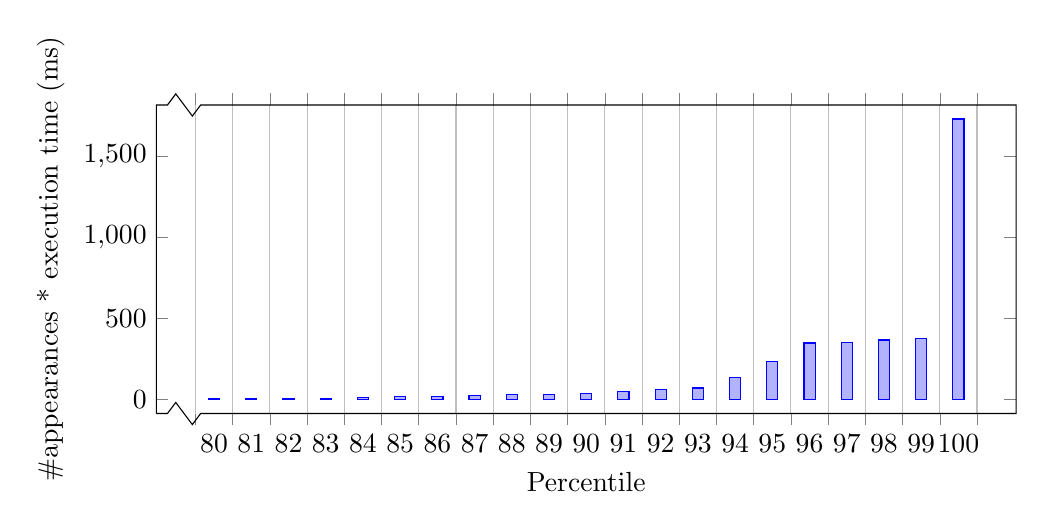
\begin{tikzpicture}
\begin{axis}[
	x tick label style={
		/pgf/number format/1000 sep=},
	ylabel=\#appearances * execution time (ms),
        xlabel=Percentile,
	enlargelimits=0.05,
	legend style={at={(0.5,-0.1)},
	anchor=north,legend columns=-1},
	ybar interval=0.3,
        axis x discontinuity=crunch
]

\addplot 
	coordinates {(80, 3.909)
            (81, 4.361) (82, 4.934)
            (83, 6.515) (84, 10.682)
            (85, 16.204) (86, 17.215)
            (87, 23.746) (88, 28.900)
            (89, 32.942) (90, 38.231)
            (91, 49.141) (92, 60.599)
            (93, 71.221) (94, 135.862)
            (95, 235.4) (96, 348.644)
            (97, 352.313) (98, 367.095)
            (99, 374.032) (100, 1731.569)
            (101, 0)};
\end{axis}
\end{tikzpicture}
\caption{Quantile performance analysis of rules using YAGO3-10 \& 107k rules}
\label{fig:quantile-analysis}
\end{figure}



The quantile analysis in \Cref{fig:quantile-analysis} is based on the number of appearances multiplied with the average execution of the rules after using the validation set as target triples as described in \ref{pre-computation}. It indicates that only few rules incur a major share of the cost. This ranking is used to determine the top x\% for the “pre-computing of expensive rules” optimization. In the given example (YAGO3-10 \& 107k rules), we achieved an 98.8\% execution time reduction for the pre-computed top 1\% rules. The pre-compution took five minutes. This reduced our average execution time from 16 ms to 10 ms, as illustrated in \Cref{tab:ablation}.


\section{Conclusions}

%
% the environments 'definition', 'lemma', 'proposition', 'corollary',
% 'remark', and 'example' are defined in the LLNCS documentclass as well.
%

We demonstrated an effective approach for finding all rules that imply a certain target fact given a knowledge graph and a set of previously learned rules. Our experiments specifically demonstrated the effect of filtering, indexing and pre-computing methods. Potential next steps include a further analysis of our approach on various datasets, a comparison of different database technologies (particularly triplestores), exploring the use of multithreading and creating a dedicated solution only using the main memory.

\textbf{Acknowledgement.} This paper would not have been possible without the exceptional support of our supervisor, Prof. Dr. Rainer Gemulla.

%%% Angabe der .bib-Datei (ohne Endung) / State .bib file (for BibTeX usage)
\bibliography{references} %\printbibliography if you use biblatex/Biber
\end{document}
